\section{Project Timeline}
The entire project consists of four phases: Repair, Design, Develop, and Teach.

\begin{figure}[h]
    \centering
    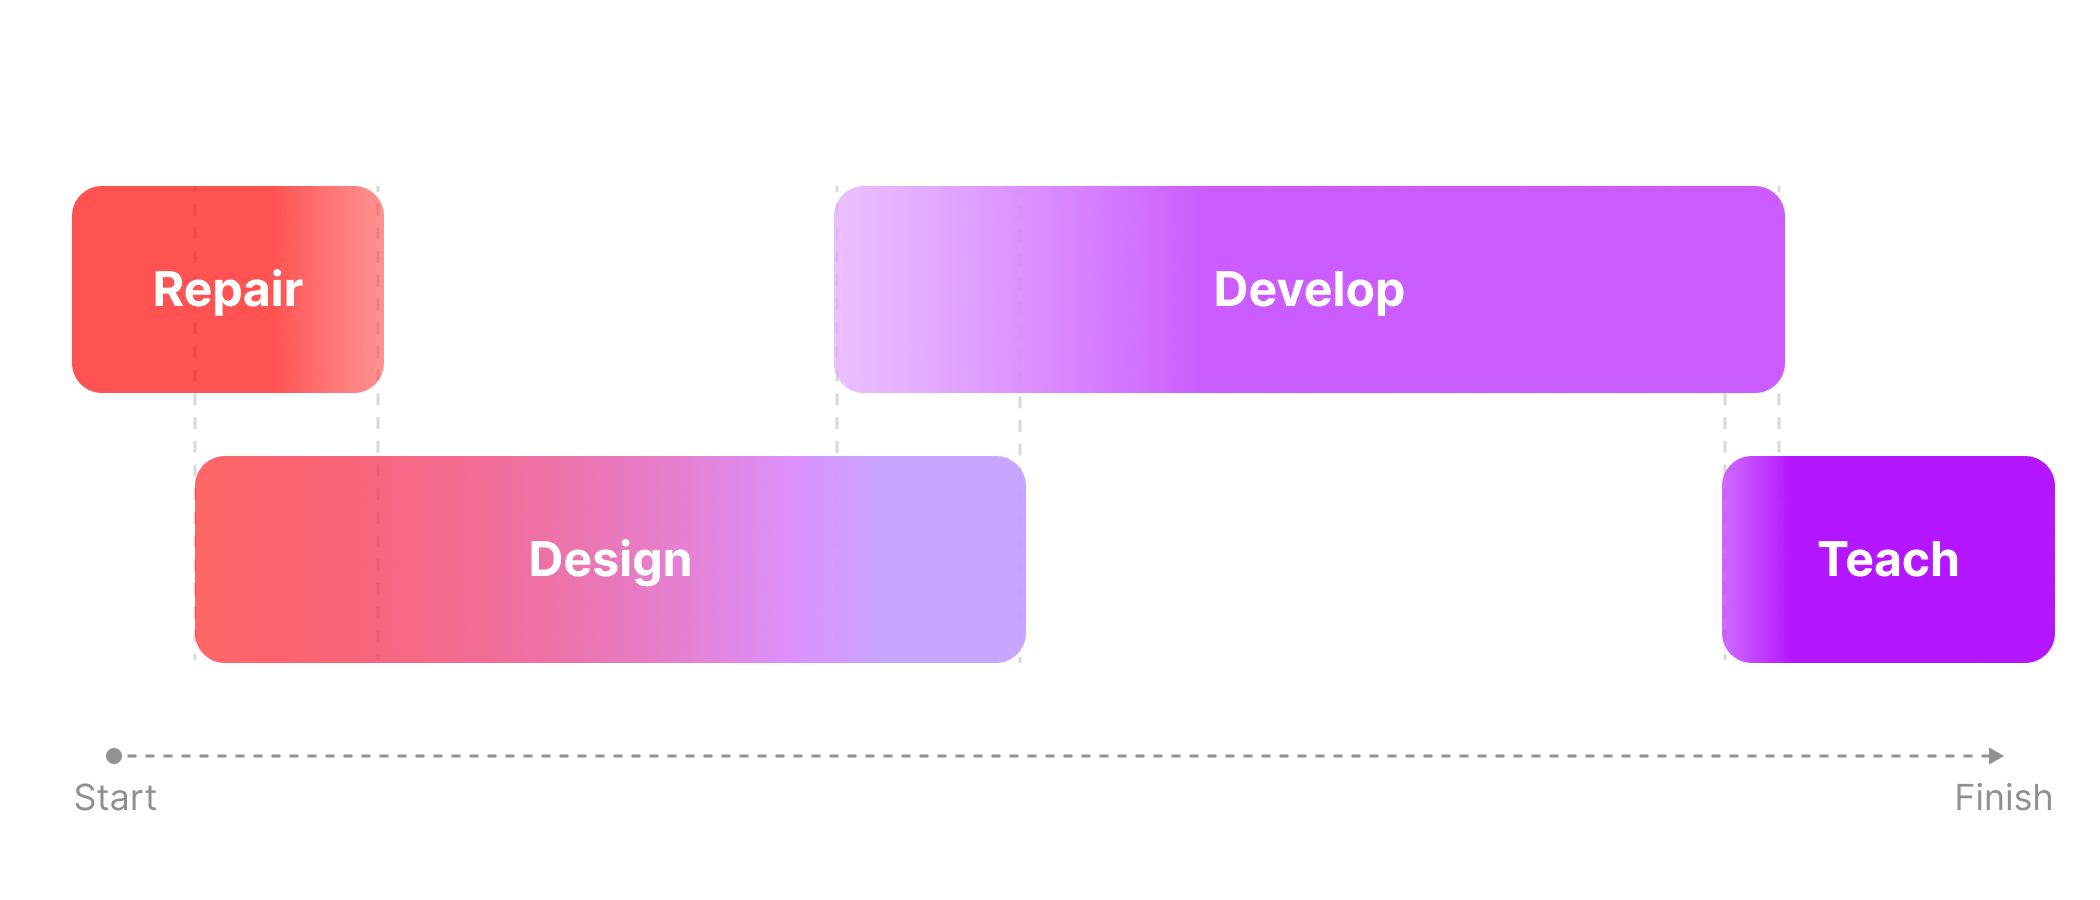
\includegraphics[scale=0.45]{diagrams/Phases.png}
    \caption{A simple graphic visualizing the phases.}
    \label{fig:phases}
\end{figure}

The actual deadlines or sequential months are not given in figure~\ref{fig:phases}. This should merely serve as a simplified timeline visualization. Note that these phases, although sequential, are also parallel. This shortens the time frame and design orientation, but requires more planning and organization.

\subsection{Repair}
This is a crucial phase that must happen as soon as possible. The goal of this phase is to fix the constant error that appears when visiting the site, as seen in figure~\ref{fig:psra}.

\begin{figure}[H]
    \centering
    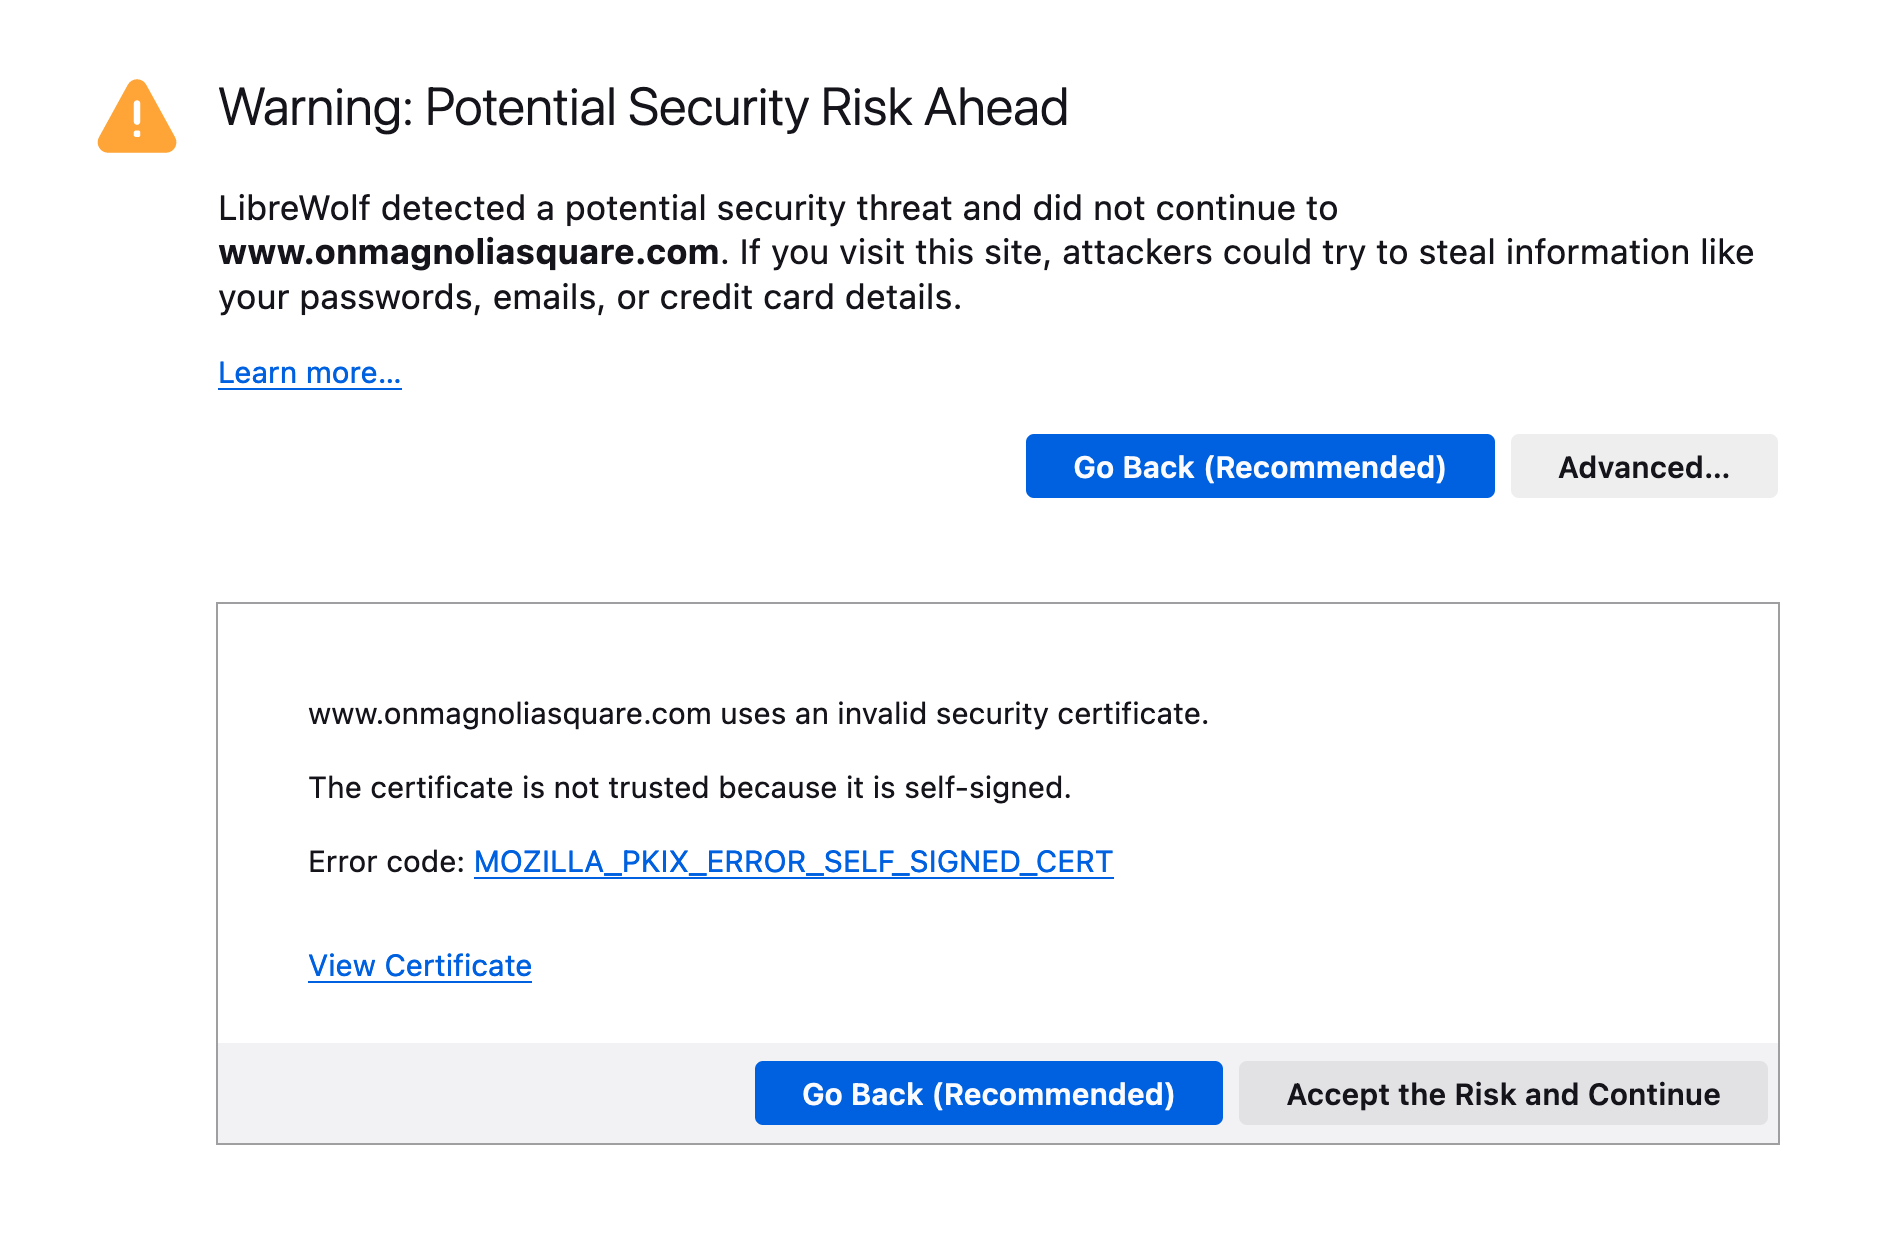
\includegraphics[scale=0.3]{pictures/securityriskahead.png}
    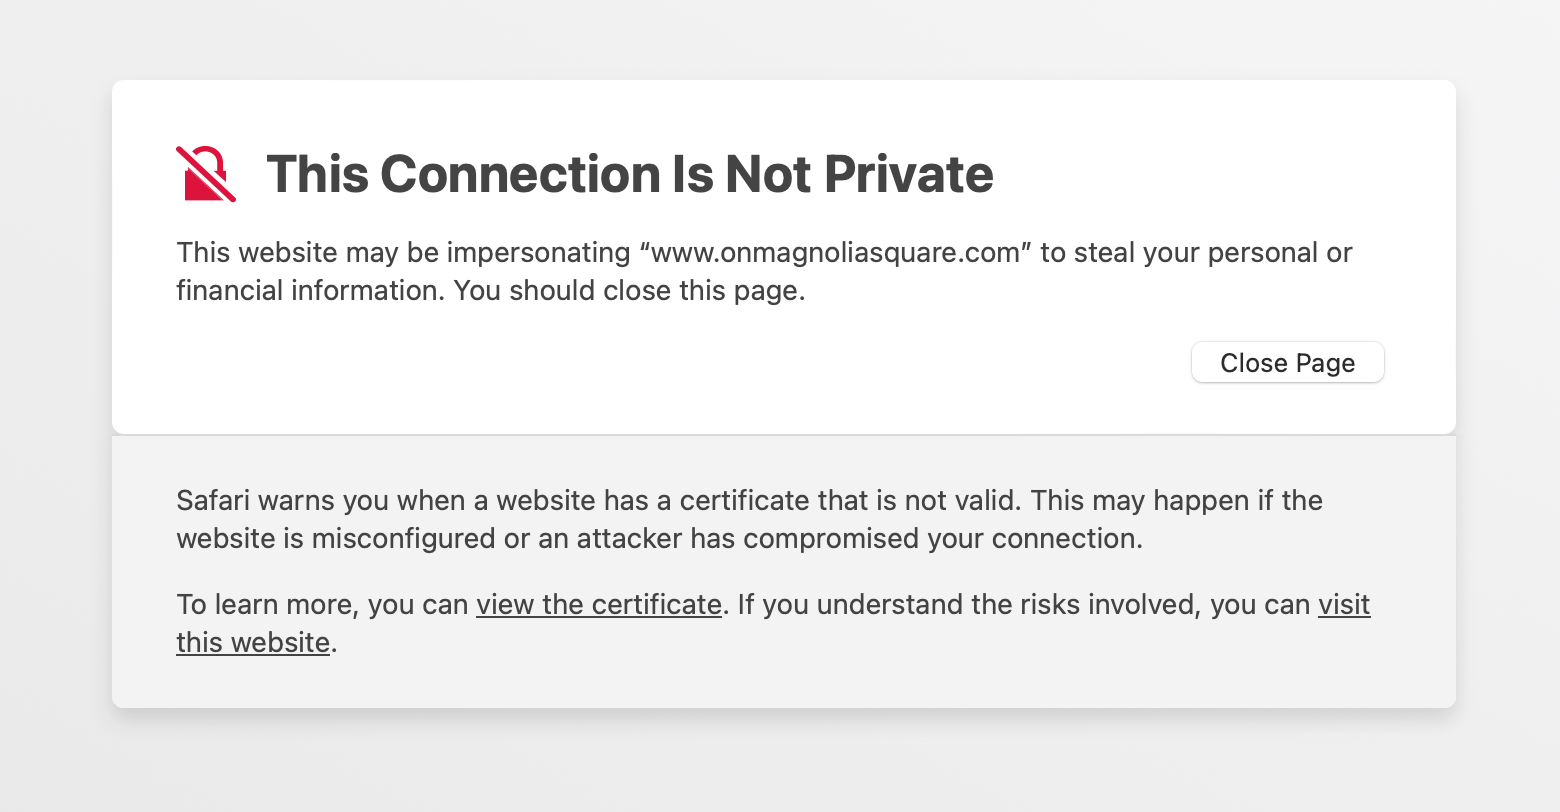
\includegraphics[scale=0.3]{pictures/potentialsecurityrisk2.png}
    \caption{Flavors of the security warning, first in Firefox and next in Safari.}
    \label{fig:psra}
\end{figure}

The issue is a website certificate error, a backend issue manifesting at the frontend. I do not yet know the reason for this error, but I am confident in my diagnosis. I have attempted to fix this error before, but my fix was unsuccessful, so moving to Cloudflare would eliminate all GoDaddy variables that may be causing the issue and expose more of the technical architecture for better surgery.

\subsubsection*{Moving to Cloudflare}
Cloudflare has a \href{https://blog.cloudflare.com/a-step-by-step-guide-to-transferring-domains-to-cloudflare/}{step-by-step guide} on their website detailing the steps and requirements to successfully switch domain registrars. In short, necessary credentials include:

\begin{itemize}
    \item Credentials for GoDaddy
    \item Payment information to authorize domain payment
    \item Credentials for onmagnoliasquare@gmail.com
\end{itemize}

These items will enable me to successfully transition our DNS Registrar from GoDaddy to Cloudflare. Transferring a domain between registrars will not affect the domain name or TLD. Those will be exactly the same.

\subsubsection*{Caveat}
Just because we change domain name registrars does not mean we are completely done with using GoDaddy in the meantime, since we still need GoDaddy to host the cPanel hosting for the Wordpress CMS. We leave GoDaddy at the end of the Develop phase.

\subsection{Design}
This phase takes place during the Fall Semester of 2023 and concludes into the middle of the Spring Semester in 2024. In this phase, we will make overhauls to the UI/UX design of the current website. It will feature a coherent experience from desktop to mobile devices, as well as compliance with web content accessibility guidelines. We will execute a UI/UX design development process, which starts with user research, to defining the problem, to actual designing, then to prototyping, then to feedback. Included in this process is the creation of usability interviews and studies, cross-platform coherent design system diagrams, and non-functional prototypes of the site itself.

\subsection{Develop}
During this phase, real world web development takes place, meaning a combination of asset and art creation, tech systems migration, and programming. The goal in this phase is to implement the new design system, to ensure technical stability across the platform for both readers and OMS members, and to start copying content from the old website to the new one. Once all content has been copied and technical stability is ensured, a transition to the new website will take place, and the old one wll be discarded. This phase will begin and end in the Spring Semester of 2024.

\subsection{Teach}
This final phase is about introducing and teaching the new website's features, functionality, and management. Teaching about these pivotal changes and functionality will occur during one or two team meetings. Due to the nature of a university student's social life and educational or non-educational commitments, I will personally reach out to those responsible for publishing content or maintaining the website in order to get them up to speed. Therefore, the meetings will be a general overview, and I will have personal meetings with respective OMS committee members for their benefit.

I will disseminate three reference documents. One with design documentation, one with development documentation, and one with general information. Design documentation will explain the website's design language and the reasons for the choices. It will also provide a guide on reasoning through a UI/UX change. Development documentation will provide future OMS developers with help with the systems architecture and lessons we will have learned from developing the website. The general information guide will be for understanding the general functioning of the website in non-technical language. It is up to future members' discretion to implement this documentation I will have created. These are merely guides.

After the project is complete, I should not have to intervene with any issues after I graduate. However, such a high stake goal does not always manifest in the way you want it to. In the case that major issues arise that would perhaps require knowledged intervention, future OMS members are always welcome to email me in the future regarding how things work. I will be glad to teach them. Graduating from NYUSH only signifies my transition from a student to a mentor. I am always willing to give back to the community that created me.
